\documentclass[master, och, pract]{SCWorks}
% Тип обучения (одно из значений):
%    bachelor   - бакалавриат (по умолчанию)
%    spec       - специальность
%    master     - магистратура
% Форма обучения (одно из значений):
%    och        - очное (по умолчанию)
%    zaoch      - заочное
% Тип работы (одно из значений):
%    coursework - курсовая работа (по умолчанию)
%    referat    - реферат
%    otchet     - универсальный отчет
%    nirjournal - журнал НИР
%    diploma    - дипломная работа
%    pract      - отчет о научно-исследовательской работе
%    autoref    - автореферат выпускной работы
%    assignment - задание на выпускную квалификационную работу
%    review     - отзыв руководителя
%    critique   - рецензия на выпускную работу
% Включение шрифта
%    times      - включение шрифта Times New Roman (если установлен)
%                 по умолчанию выключен
\usepackage{preamble}

\begin{document}

% Кафедра (в родительном падеже)
\chair{Информатики и программирования}

% Тема работы
\title{Разработка платформы единого резюме}

% Курс
\course{2}

% Группа
\group{273}

% Факультет (в родительном падеже) (по умолчанию "факультета КНиИТ")
% \department{факультета КНиИТ}

% Специальность/направление код - наименование
% \napravlenie{02.03.02 "--- Фундаментальная информатика и информационные технологии}
\napravlenie{02.04.03 "--- Математическое обеспечение и администрирование информационных систем}
% \napravlenie{09.03.01 "--- Информатика и вычислительная техника}
% \napravlenie{09.03.04 "--- Программная инженерия}
% \napravlenie{10.05.01 "--- Компьютерная безопасность}

% Для студентки. Для работы студента следующая команда не нужна.
% \studenttitle{Студентки}

% Фамилия, имя, отчество в родительном падеже
\author{Кулакова Максима Сергеевича}

% Руководитель НИР
\nirtitle{к.\,э.\,н., доцент} % степень, звание
\nirname{Л.\,В.\,Кабанова}

% Заведующий кафедрой
\chtitle{к.\,ф.-м.\,н.} % степень, звание
\chname{М.\,В.\,Огнева}

% Научный руководитель (для реферата преподаватель проверяющий работу)
\satitle{к.\,э.\,н., доцент} %должность, степень, звание
\saname{Л.\,В.\,Кабанова}

% Руководитель практики от организации (только для практики, для остальных типов
% работ не используется)
\patitle{к.\,э.\,н., доцент}
\paname{Л.\,В.\,Кабанова}

% Семестр (только для практики, для остальных типов работ не используется)
\term{1}

% Наименование практики (только для практики, для остальных типов работ не
% используется)
\practtype{производственная (научно-исследовательская работа)}

% Продолжительность практики (количество недель) (только для практики, для
% остальных типов работ не используется)
\duration{18}

% Даты начала и окончания практики (только для практики, для остальных типов
% работ не используется)
\practStart{01.09.2023}
\practFinish{14.01.2024}

% Год выполнения отчета
\date{2024}

\maketitle

% Включение нумерации рисунков, формул и таблиц по разделам (по умолчанию -
% нумерация сквозная) (допускается оба вида нумерации)
\secNumbering

\tableofcontents

% Раздел "Обозначения и сокращения". Может отсутствовать в работе
% \abbreviations
% \begin{description}
%     \item ... "--- ...
%     \item ... "--- ...
% \end{description}

% Раздел "Определения". Может отсутствовать в работе
% \definitions

% Раздел "Определения, обозначения и сокращения". Может отсутствовать в работе.
% Если присутствует, то заменяет собой разделы "Обозначения и сокращения" и
% "Определения"
% \defabbr

% Ссылка на источник в тексте
% \cite{}





\intro
Современная веб-разработка требует надежных, интерактивных и масштабируемых решений, одним из которых является клиент-серверная разработка. Данная архитектура не только обеспечивает эффективное управление получаемыми и обрабатываемыми данными, но и позволяет организовать бесперебойную работу со множеством пользователей.

На данный момент существует множество мощных инструментов, способных разработать веб-приложение, соответствующее всем необходимым минимальным требованиям. Одними из таких популярных разработок являются ReactJS для разработки надежных динамических пользовательских интерфейсов на основе виртуального DOM, архитектурное решение REST API, прекрасно дополняющий и обеспечивающий стандартизированный подход к разработке веб-сервисов, и TailWindCSS, способный заменить неоптимизированное стилевое оформление в более приятные компоненты.

Разработчики могут обеспечить масштабируемость, модульность и совместимость своих приложений, придерживаясь принципов REST. 

Цель научно-исследовательской работы заключается в масштабировании платформы создания единого резюме до клиент-серверного приложения.

Задачами работы являются следующие пункты: 
\begin{enumerate}
    \item Обзор технических средств реализации приложения, включающий в себя React, Next JS, TailWind, Rest API;
    \item Настройка конфигурации основного функционала приложения;
    \item Реализация взаимодействия платформы с существующими сервисами по API;
    \item Подведение итогов проведенной научно-исследовательской работы.
\end{enumerate}




% После введения — серии \section, \subsection и т.д.
\newpage
\section{Теоретические аспекты разработки}
\subsection{Интерфейсная библиотека React JS}
React JS - это библиотека JavaScript с открытым исходным кодом, которая предназначена для разработки пользовательских интерфейсов веб-приложений, особенно для интерактивных веб-страниц. Она позволяет использовать "компоненты", которые являются маленькими блоками кода, для создания сложных пользовательских интерфейсов.

React JS прост и удобен в эксплуатации. Понимание основных требований практически не требует времени и может быть выполнено в течение нескольких часов. Разработчики предпочитают использовать React JS по следующим причинам:
\begin{enumerate}
    \item Динамические приложения требуют более сложного кодирования, и использование React JS упрощает данную задачу;
    \item Возможность повторного использования компонентов. В React очень тесно связаны разметка и логика, благодаря чему появляется возможность хранить все данные о внешнем виде компонента и его изменения в процессе работы в одном файле;
    \item Использование виртуального дерева вместо физического для повышения производительности будущего приложения. Для JavaScript структура dom-дерева является интерфейсом, через который скрипты приводят в движение html и css-объекты, поэтому производительность в данном случае играет очень значимую роль;
    \item Снижается нагрузка на сервер и время разработки. Повышается производительность сайта: быстрее открываются страницы и отзывается на действия пользователей интерфейс;
    \item По сравнению с обычными сайтами у сайтов на React более чистая архитектура, в которой проще обнаруживать и исправлять баги и которую проще поддерживать. \cite{rjs_vs_rn}\cite{rjs}
\end{enumerate}

Фреймворк React использует JSX, расширение для языка JavaScript, представляя все HTML-элементы интерфейса в роли компонентов, используя подход «разделяй и властвуй», упрощая разработку проекта, особенно удобно для командной разработки. Подобный подход используется во всех современных фреймворках для разработки динамического web-интерфейса\cite{Ershov_web}.

React очень удобно рассматривать для разработки одностраничных приложений. Несмотря на то, что при снятии нагрузки с сервера нагружается его клиентская часть, современные браузеры способны справиться с отрисовкой страниц благодаря достаточному запасу памяти и подхода SPA. Его суть в том, что весь сайт — это одна страница, которую React постоянно перерисовывает – но не целиком. Если в одностраничных страницах есть возможность оптимизации ресурсов, то и в многостраничных решениях оно будет присутствовать вдоволь.

В простом приложении для перехода со страницы на страницу пользователь делает к ней запрос на сервер, и сервер возвращает разметку, стили и файлы скриптов. В случае одностраничных приложений пользователь, переходя между разделами сайта, формально находится на одной и той же странице, но файлы скриптов и стили у него уже есть — остается догрузить то, чего не хватает. 

По состоянию на конец 2023 года React находится в лидирующих позициях среди JavaScript-технологий для разработки фронтенда\cite{rjs}.




\subsection{Серверная библиотека NextJS}
Переходя к основоположникам применения серверных компонентов можно отнести создателей средства Next.js, развивающих упомянутую концепцию. Next.js – это фреймворк, основанный на React, который позволяет создавать веб-приложения с улучшенной производительностью, используя рендеринг на серверной стороне\cite{Cheprasov}.

Дополнительный функционал NextJS обеспечивает реализацию оптимизированных и полезных возможностей, таких как:
\begin{enumerate}
    \item Server Side Rendering – позволяет рендерить полноценную страницу на сервере, после чего она полностью отправляется на клиентскую часть и сразу же отображается, что повышает производительность веб-страниц;
    \item Search Engine Optimization – помогает веб-приложению занимать более высокие места в поисковых системах. SEO работает в тандеме с SSR и позволяет трекерам сканировать больше контента;
    \item Упрощенный процесс разворачивания приложения\cite{Nikitin_nextjs}.
\end{enumerate}

Next.js может быть использован для разработки клиент-серверных приложений с улучшенной производительностью и возможностью использования серверного рендеринга. В качестве фреймворка, основанного на React, Next.js предоставляет средства для создания веб-приложений, которые взаимодействуют с сервером. Он обеспечивает серверный рендеринг, что означает, что приложение может получить полноценную HTML-страницу на сервере и отправить ее на клиентскую сторону для отображения. Это позволяет повысить производительность сайта и улучшить SEO-оптимизацию.

Следовательно, основные подходы к использованию Next.js для разработки клиент-серверных приложений включают в себя применение серверного рендеринга для оптимизации производительности, управление маршрутизацией, обработку данных на стороне сервера, а также управление локальным состоянием приложения.




\subsection{Интерфейсная библиотека TailWind}
TailwindCSS является набирающим популярность CSS-фреймворком, который дает возможность вносить изменения в оформление сайтов и приложений, не покидая HTML-разметку, в том числе и в компонентах React, не используя тег style. Эти служебные классы позволяют инкапсулировать общие шаблоны стилей, такие как поля, отступы, цвета и макеты флексбоксов, что позволяет быстро создавать и настраивать пользовательский интерфейс\cite{Tailwind}.

Одним из ключевых преимуществ является гибкость и расширяемость. Фреймворк предоставляет широкие возможности настройки, позволяющие разработчикам настраивать структуру в соответствии с конкретными требованиями проекта. Эта гибкость делает его подходящим для широкого спектра проектов: от небольших личных веб-сайтов до крупномасштабных корпоративных приложений.

TailwindCSS является его ориентация на производительность и оптимизацию. Используя служебные классы, разработчики могут избежать раздувания, которое часто возникает при использовании традиционных платформ CSS, что приводит к меньшим размерам файлов CSS и более быстрому времени загрузки. Более того, поощряет модульный подход к стилизации, который может привести к созданию более удобных в обслуживании и масштабируемых баз кода.

Несмотря на свой подход, ориентированный на полезность, Tailwind CSS не жертвует гибкостью дизайна. Платформа предоставляет полный набор служебных классов, которые охватывают широкий спектр вариантов стилей, что позволяет разработчикам с легкостью создавать визуально привлекательные и адаптивные проекты. Кроме того, Tailwind CSS легко интегрируется с популярными интерфейсными платформами, такими как React, Vue.js и Angular, что упрощает его включение в существующие проекты\cite{Fain_2022}.

Основными преимуществами TailWindCSS являются следующие возможности:
\begin{enumerate}
    \item Наличие базовых классов для оформления страниц. В библиотеке есть базовый конфигурационный файл, и в него по умолчанию включена большая коллекция классов, необходимых для стилизации приложения, таких как flex, grid, block для display, m-10 вместо margin и подобных;
    \item Наличие расширенной цветовой палитры. Цвета здесь имеют привычные названия и постфикс с насыщенностью в цифровом обозначении, например, red-50 будет являться бледно-розовым цветом, когда red-900 уже приобретет более бордовый оттенок;
    \item Продвинутые CSS-свойства. Различные анимации, радиусы закругления рамок, повороты, отступы;
    \item Переменные. Помимо классов, в TailwindCSS есть и переменные в стиле тех, что используется в CSS-препроцессорах. С помощью них можно уложить несколько классов в один и использовать его как классический семантический селектор. Делается это с помощью директивы @apply;
    \item Добавление собственных классов. В этом плане Tailwind можно настроить под индивидуальные требования и предпочтения. Для этого требуется прописать новые свойства в конфигурационный файл фреймворка\cite{Tailwind}.
\end{enumerate}

Подводя итог, Tailwind CSS предлагает современный и эффективный подход к стилизации веб-приложений. Благодаря своей философии приоритета полезности, широким возможностям настройки и ориентации на производительность дает разработчикам возможность создавать красивые и отзывчивые пользовательские интерфейсы с меньшими усилиями и большей гибкостью\cite{Rifandi_2022}. 




\subsection{Архитектурный стиль Rest API}
Rest API - это интерфейс программирования приложений, основанный на принципах REST. Web API или Web Service API –это интерфейс обработки приложений между веб-сервером и веб-браузером. Все веб-сервисы являются api, но не все api являются веб-сервисами. Rest API – это особый тип Web API, в котором используется стандартный архитектурный стиль, описанный выше\cite{Kalinin_mic}.

Различные термины, которые относятся к API, например, Java API или сервисные API, существуют в связи с исторически ранним происхождением, тк API-архитектуры начали появляться до запуска Всемирной паутины. Современные web API – это REST API, и эти термины могут использоваться взаимозаменяемо.

Данный архитектурный стиль стал популярным из-за своей простоты, гибкости и масштабируемости. Он использует стандартные HTTP-методы, такие как GET, POST, PUT и DELETE, для работы с ресурсами на сервере. Каждый ресурс имеет уникальный идентификатор, с которым клиенты могут взаимодействовать.

В качестве основных преимуществ архитектурного стиля Rest API можно выделить следующие ключевые моменты:
\begin{enumerate}
    \item Гибкость – позволяет разработчикам использовать различные форматы данных, такие как json или html. Это позволяет клиентам и серверам обмениваться данными в удобном для них формате;
    \item Простота – использует стандартные HTTP-методы, что делает его простым в использовании и понимании. Разработчики могут легко создавать, изменять и расширять api без необходимости в специальных инструментах или библиотеках;
    \item Масштабируемость – позволяет разрабатывать распределенные системы, где клиенты и серверы могут находиться на разных компьютерах или даже в разных частях мира. Это делает его идеальным для создания клиент-серверных приложений;
    \item Кэширование – поддерживает кэширование данных на клиентской стороне, что позволяет улучшить производительность и снизить нагрузку на сервер;
    \item Независимость от платформы – не привязан к определенной платформе или языку программирования. Это означает, что клиенты и серверы могут быть реализованы на различных технологиях, а это уже обеспечивает большую гибкость и возможность использования уже существующих разработанных систем.\cite{Masse_rest}
\end{enumerate}

В настоящее время Rest API является широко используемым и популярным подходом для разработки клиент-серверных приложений, благодаря своей простоте, гибкости, масштабируемости и прочим незаменимым, полезным возможностям.






\section{Реализация платформы единого резюме}
\subsection{Общие настройки динамического приложения}
Для компенсации недостатков статических сайтов и динамической генерации страниц из набора входящих параметров и данных инициализируем проект с NextJS и добавим интерфейсную библиотеку NextUI для удобства разработки следующими командами:
\begin{minted}[fontsize=\small, breaklines=true, style=bw, linenos]{bash}
npx create-next-app@latest
npm i @nextui-org/react framer-motion
\end{minted}

Для безопасной работы с проектом необходимо создать файл process.env, в котором будут хранится переменные окружения, например токен доступа к системе.

Дополнительно для каждой страницы необходимо задать общий шаблон в файле layout.tsx, находящимся в корневой папке приложения. Данная структура представляет из себя обёртку над стандартным представлением HTML файла, внутрь которого добавлено реактивное представление. Дополнительно внутри атрибутов указываются стили для блоков, такие как минимальная высота контейнера, цвет фона, размеры контейнеров, отступов и их поведение, выбор шрифта и текущая цветовая схема. В дальнейшем содержимое атрибутов className будет  игнорироваться. 
\begin{minted}[fontsize=\small, breaklines=true, style=bw, linenos]{text}
export default function RootLayout({ children, }:{
	children: React.ReactNode;
}) { return (
<html lang="en" suppressHydrationWarning>  
    <head></head>
    <body className={clsx( "min-h-screen bg-background font-sans antialiased", fontSans.variable )}>
    <Providers themeProps={{ attribute: "class", defaultTheme: "dark" }}>
    <div className="relative flex flex-col h-screen">
    <Navbar/>
    <main className="container mx-auto max-w-7xl pt-16 px-6 flex-grow">
    {children}
    </main></div></Providers></body>
</html>
);}
\end{minted}




\subsection{Написание механизма авторизации}
Для реализации авторизации создадим файл auth.ts, в котором укажем конфигурацию с сервисом Github посредством открытого протокола безопасности OAuth и с классической проверкой логина и пароля. Для этого создадим два соответсвующих свойства и в первое передадим переменные приложения для авторизации через сторонний сервис, а в втором реализуем проверку введённых в поля данных и в случае соответсвия вернём самого пользователя с его именем, фотографией профиля и ролью\cite{Fain_2022}.
\begin{minted}[fontsize=\small, breaklines=true, style=bw, linenos]{text}
export const authConfig: AuthOptions = { providers: [
    GithubProvider({
        clientId: process.env.GITHUB_ID!,
        clientSecret: process.env.GITHUB_SECRET!,}),
    Credentials({
    credentials: {
        email: { label: 'email', type: 'email', required: true },
        password: { label: 'password', type: 'password', required: true }, },
        async authorize(credentials) {
        if (!credentials?.email || !credentials.password) return null;
        const currentUser = users.find(user => user.email === credentials.email)
        if (currentUser && currentUser.password === credentials.password) {
            const { password, ...userWithoutPass } = currentUser;
            return userWithoutPass as User;}
    return null }})
    ], pages: { signIn: '/signin' } }
\end{minted}

Ограничение доступа неавторизованного пользователя к внутренним и закрытым страницам достигается созданием файла middleware.ts, в котором через параметры указываются пути навигации и, в случае попадания в заданный путь, перевод клиента на страницу signIn.
\begin{minted}[fontsize=\small, breaklines=true, style=bw, linenos]{text}
export const config = { matcher: ['/profile/:path*', '/hh', 
    '/resume','/protected/:path*'] }
\end{minted}

Дополнительно к предыдущему пунту контроля доступа опишем корневой файл providers.tsx, созданный для окружения корневого элемента страницы в её компоненты, свойства стилей и сессию пользователя.
\begin{minted}[fontsize=\small, breaklines=true, style=bw, linenos]{text}
export function Providers({ children, themeProps }: ProvidersProps) {
return (
<SessionProvider><NextUIProvider>
    <NextThemesProvider {...themeProps}>
        {children}
    <NextThemesProvider>
<NextUIProvider><SessionProvider>);}    
\end{minted}

Процесс авторизации реализуется на клентской и серверной части приложения, поэтому для корректного взаимодействия необходимо создать обработчик событий по API в динамическом маршруте [..auth]/route.tsx с следующими параметрами:
\begin{minted}[fontsize=\small, breaklines=true, style=bw, linenos]{text}
const handler = NextAuth(authConfig);
export { handler as GET, handler as POST }
\end{minted}

Реализуем форму авторизации через компонент SignInForm с двумя текстовыми формами, для этого
инициализируем роутер переходов, обратные вызовы для динамического контента и обработчик нажатия кнопки отправки формы, получающий данные полей и выполняющий вход в систему.
\begin{minted}[fontsize=\small, breaklines=true, style=bw, linenos]{text}
const SignInForm = () => {
    const router = useRouter();
    const [isVisible, setIsVisible] = React.useState(false);
    const toggleVisibility = () => setIsVisible(!isVisible);
    const handleSubmit: FormEventHandler<HTMLFormElement> = async (event) => {
        event.preventDefault();
        const formData = new FormData(event.currentTarget);
        const res = await signIn("credentials", {
            email: formData.get("email"),
            password: formData.get("password"),
            redirect: false
\end{minted}

Кнопка авторизации через Github работает через параметры поисковой строки, получаемые в процессе возврата на страницу платформы после успешного входа на стороне внешнего сервиса.
\begin{minted}[fontsize=\small, breaklines=true, style=bw, linenos]{text}
export const GithubButton = () => {
const searchParams = useSearchParams();
const callbackUrl = searchParams.get("callbackUrl") || "/profile";
return (
    <Button onClick={() => signIn("github", { callbackUrl })}>        
        Log In with GitHub
    </Button>
);};
\end{minted}

После написания компонентов необходимо создать саму страницу авторизации, для этого внутрь всей иерархической оболочки страниицы передадим заголовок вместе с компонентами SignInForm и GithubButton, после которых страница будет располагаться по маршруту app/signIn. Итоговый вид страницы авторизации отображён на рисунке~\ref{fig:1}. 
\begin{figure}[!ht]
    \centering
    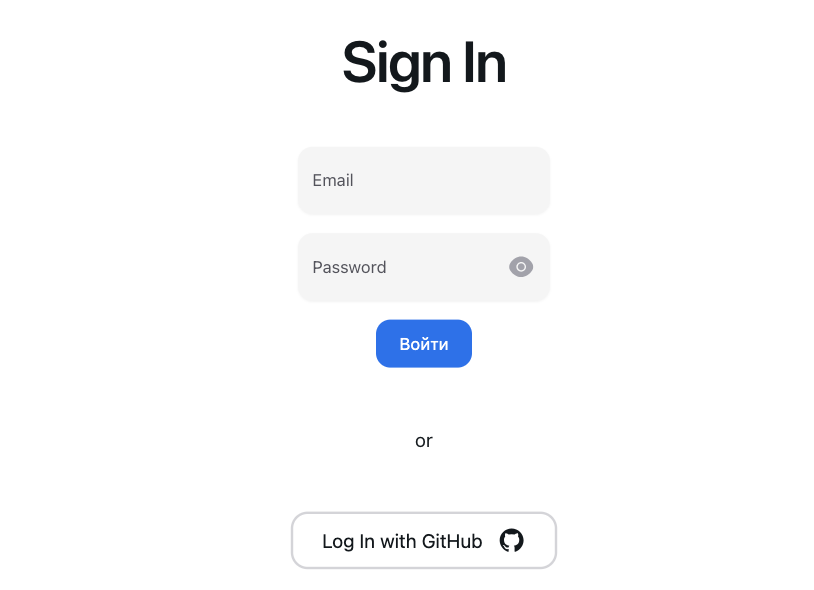
\includegraphics[width=12cm]{images/image-signin.png}
    \caption{\label{fig:1}%
        Страница авторизации}
\end{figure}




\subsection{Реализация страницы резюме}
Для написания модуля необходимо создать структуру данных резюме. Информация о профиле хранится в формате текстовом формате обмена данными JSON и содержит в себе следующие поля:
\begin{enumerate}
    \item Id -- генерируемый уникальный идентификатор резюме;
    \item Name -- фамилия и имя человека;
    \item Description -- краткое описание профиля;
    \item Social links -- ссылки на социальные сети;
    \item Profile image -- изображение работника для резюме;
    \item About -- текстовое поле с рассказом о себе, являющееся аналогом сопроводительного письма;
    \item Education, experience -- группы образования и опыта работы, включающие в себя следующие пункты:
    \begin{enumerate}
        \item Name -- наименование места работы или учебного учереждения;
        \item Description -- описание чем занимался соискатель в данное время;
        \item Start date, end date -- дата начала и окончания; 
        \item Current date -- поле, показывающее что дата окончания отсутвует и при подсчёте её следует считать текущим днём;
    \end{enumerate}
    \item Projects -- поле проектов, следующее из опыта работы. Включает в себя:
    \begin{enumerate}
        \item Name -- наименование проекта;
        \item Description -- описание проекта и над чем происходила работа;
        \item Image -- изображение проекта, его логотип, интерфейс.
    \end{enumerate}
\end{enumerate}

Последовательно реализуем компоненты, начиная с блока контактов и ссылок на социальные сети, получающий на вход список адресов и возвращающий горизонтальный список кнопок с переходом и миниатюрами соответвующих сервисов. Изображения предварительно описываются в формате svg в компоненте icons.tsx, после чего из строки выделяется имя хостинга с последующим добавлением в массив элементов для отображения на странице.
\begin{minted}[fontsize=\small, breaklines=true, style=bw, linenos]{text}
function IconVariant(service: string, icon_color:string, icon_size:number) {
switch(service) { 
    case "github.com": 
        { return <GithubIcon className={icon_color} size={icon_size}/>; } 
    default: 
        { return <InternetIcon className={icon_color} size={icon_size}/>; }
}};
export const SocialLink = (props : SocialProps) => {
    const icon_size, icon_color = 36, "text-default-500";
    const social_icons = props.links.map((element, index) => {
    var url = new URL(element.toString());
return 	
    <Link isExternal href={element.toString()} key={index}>
        {IconVariant(url.host.toString(), icon_color, icon_size)}
    </Link>;
});};
\end{minted}

Итоговый вид компонента показан на рисунке~\ref{fig:2}. 
\begin{figure}[!ht]
    \centering
    
\includegraphics[width=12cm]{images/image-resume-1.png}
    \caption{\label{fig:2}%
        Компонент отображения контактов и ссылок}
\end{figure}

Опишем компонент вывода образования и опыта работы. Для этого реализуем функционал подсчёта текущего затраченного времени через получение двух строковых и одной логической переменных из файла резюме, преобразования текста в объект даты и нахождения разницы между двумя величинами. После вычисления необходимо округлить полученное значение до целого числа и преобразовать в удобочитаемый внешний вид с помощью проверки количества месяцев и лет. Результатом работы функций станет вывод временного значения в строке компонента. Полный код реализации компонента можно найти в приложении А.
\begin{minted}[fontsize=\small, breaklines=true, style=bw, linenos]{text}
function diffDates(day_one:any, day_two:any) {
    return (day_one - day_two) / (60 * 60 * 24 * 1000);
};
function getFormatedStringFromDays(numberOfDays:number) {
    var months = Math.floor(numberOfDays % 365 / 30);
    var yearsDisplay = years > 0 ? 
        years + (years == 1 ? " year " : " years ") : "";
    return yearsDisplay + monthsDisplay; 
};
export const Experience = (props : ExperienceProps) => {
const experience_item_list = props.experience_list.map((element, index)=>{
    return { getFormatedStringFromDays(diffDates(element.start_date, element.end_date))}})
return  <>{experience_item_list}</>
};
\end{minted}

Итоговый вид компонента показан на рисунке~\ref{fig:3}.  
\begin{figure}[!ht]
    \centering
    
\includegraphics[width=12cm]{images/image-resume-2.png}
    \caption{\label{fig:3}%
        Компонент отображения опыта работы и образования}
\end{figure}

Для реализации портфолио в шахматном представлении воспользуемся классовыми атрибутами сетки из библиотеки Tailwind. Получим порядковый индекс списка проектов, начинающийся с нуля, и дальше в зависимости от чётности раздельно и поочерёдно позиционируем текст с 1 по 6 колонку и изображение с 7 по 13.
\begin{minted}[fontsize=\small, breaklines=true, style=bw, linenos]{text}
export const Projects = (props : ProjectsProps) => {
const projects = props.projects_list.map((element, index) => {
    var position_image = index % 2 == 0 ? 
        "col-start-7 col-end-13" : "col-start-1 col-span-6 ";
    var position_text = index % 2 == 0 ? 
        "col-start-1 col-end-6" : "col-start-8 col-end-13 order-1";
    return (
        <div className={position_text}>
            <h2>{element.name}</h2>
            <p>{element.description}</p>
        </div>
        <Image className={position_image}/>
    )})
return <>{projects}</>
};
\end{minted}

Итоговый вид компонента списка проектов показан на рисунке~\ref{fig:4}. 
\begin{figure}[!ht]
    \centering
    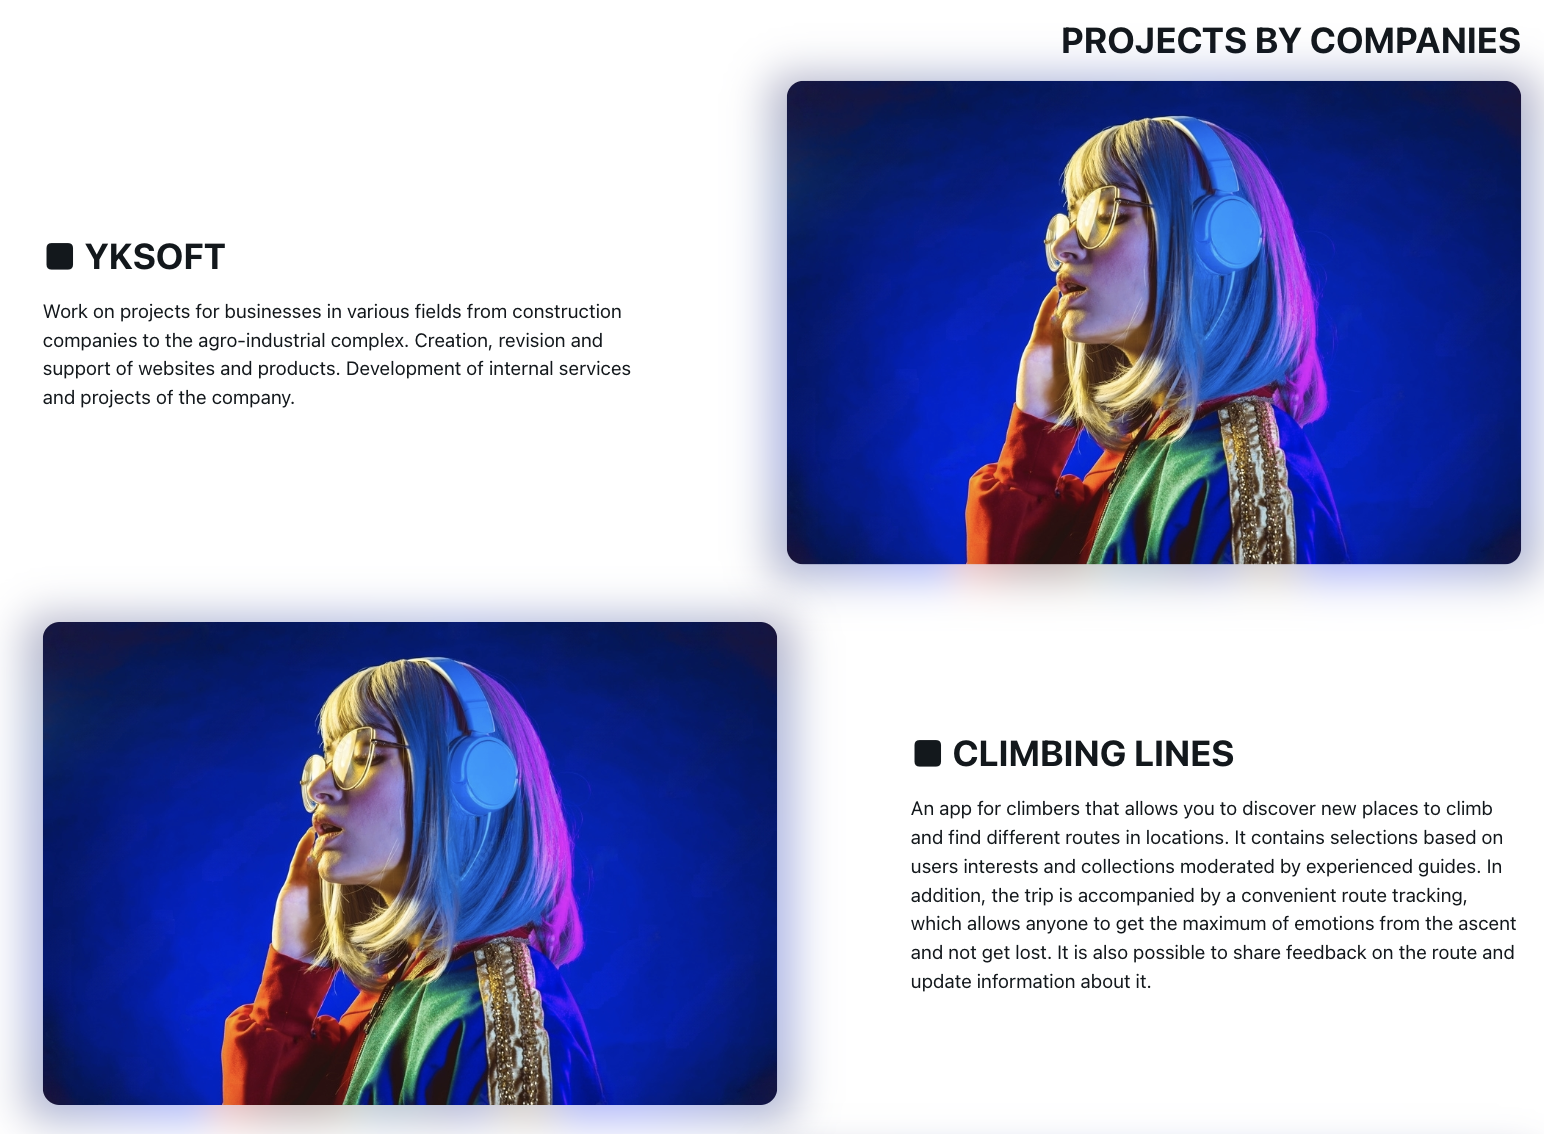
\includegraphics[width=12cm]{images/image-resume-3.png}
    \caption{\label{fig:4}%
        Компонент отображения списка проектов}
\end{figure}

После описания компонентов реализуем страницу резюме, для этого необходимо произвести запрос данных резюме и передать его поля в соответвующие теги и компоненты. Полный код реализации страницы можно найти в приложении Б.  
\begin{minted}[fontsize=\small, breaklines=true, style=bw, linenos]{text}
export default function Template1Page() {
const profile_data = require("@/data-template/template-1-data.json");
return (
<SocialLink links = {profile_data.social_links}/>
<div className="container pt-5 pb-5">
    <h2 id="projects">projects by companies</h2>
    <Projects projects_list={...profile_data.projects}/>
</div>
);}    
\end{minted}




\subsection{Взаимодействие с сервисом hh.ru}
Реализуем взаимодействие пользователя с сервисов hh.ru через API. Первоначальная конфигурация в виде авторизации состоит из 3 этапов:
\begin{enumerate}
    \item Перенаправление пользователя по адресу сервиса с переданными параметрами строки;
    \item Получение временного кода авторизации;
    \item Обмен кода авторизации на долгосрочный токен доступа к профилю и кода обновления токена в случае необходимости.\cite{hh_api}
\end{enumerate}

Первый этап достигается с помощью передачи параметров строки запроса через вопросительный знак, имя параметра и значение. В ответ на полученную от сервиса hh.ru ссылку с переходом необходимо обработать ответный параметр временного кода авторизации и обмена на долгосрочный. Опишем данный функционал в api/hh/route.tsx, для этого необходимо реализовать GET запрос, предварительно считывающий строку запроса и параметр code, в заголовок которого добавляем желаемое действие, открытый и секретный идентификаторы приложения и полученный на предыдущем обработчике код. Так как функция запросов асинхронна – воспользуемся обработчиком событий и через ожидающий обратный вызов функции передадим запрос по адресу сервиса, получив в ответ необходимый набор данных: ответ об успешности запроса и токены\cite{Razin_2020}.
\begin{minted}[fontsize=\small, breaklines=true, style=bw, linenos]{text}
export async function GET(req: Request) {
const { searchParams } = new URL(req.url)
const code = searchParams.get('code');
if (code != null) {
    myHeaders.append("Content-Type", "application/x-www-form-urlencoded");
    urlencoded.append("grant_type", "authorization_code");
    urlencoded.append("client_id", process.env.HH_ID!);
    urlencoded.append("client_secret", process.env.HH_SECRET!);
    urlencoded.append("code", code!);
    try {
        const res = await fetch("https://hh.ru/oauth/token", {
            method: 'POST', headers: myHeaders,
            body: urlencoded, redirect: 'follow' });   
        const result = await res.json();
        return NextResponse.json(result);
}} 
\end{minted}

После получения долгосрочного токена для конкретного пользователя, у приложения появляется возможность воспользоваться доступом к сервису hh.ru. Получим все существующие резюме человека и выведем их на страницу. Для этого отправим GET запрос с токеном авторизации по заданному маршруту и вернём данные в формате JSON.
\begin{minted}[fontsize=\small, breaklines=true, style=bw, linenos]{text}
const token = searchParams.get('token');
if (token != null) {
    var myHeaders = new Headers();
    myHeaders.append("Authorization", `Bearer ${token}`);
    try {
        const res = await fetch("https://api.hh.ru/resumes/mine", {
            method: 'GET', headers: myHeaders, redirect: 'follow' });      
        const result = await res.json();
        return NextResponse.json(result);
}}
\end{minted}




\subsection{Реализация страниц сравнения и обновления резюме}
Страница сравнения навыков представляет из себя таблицу, содержащую наименование поля, значения совпадающих ключей для каждого из входных резюме и поле взаимодействие, содержащее возможность добавления собственного значения, а также удаления строки. Так как резюме содержит в себе значениях разных типов, их отображение будет возможно только при сепарации. Для этого реализуем компонент сравнения, получающий значение свойства из JSON и далее в случае одиночной строки возвращающий тег с его содержимым, в случае списка строк обрабатывающий каждую из них, присваивающую уникальный индекс отображения, а в случае более глубокой вложенности добавляющей перед элементом его наименование.
\begin{minted}[fontsize=\small, breaklines=true, style=bw, linenos]{text}
if (typeof props.cv_editor == "string") {
    cv_editor_item_list = <div>{props.cv_editor}</div>;
} else {
    Object.keys(props.cv_editor).map((element, index) => {
    let arrObj = props.cv_editor[element];
    if (typeof arrObj == "object") {
    cv_editor_item_list = props.cv_editor.map((element: any, index:any) => {
    return (
        {Object.keys(element).map((el, index) => {
        return( <div key={index}>{el}: {element[el]}</div> );})}
    );});  
    } else {
        cv_editor_item_list = props.cv_editor.map((element: any, index:any) => 
        { return {element}; })
}});}
\end{minted}

Итоговый вид страницы сравнения навыков показан на рисунке~\ref{fig:5}. 
\begin{figure}[!ht]
    \centering
    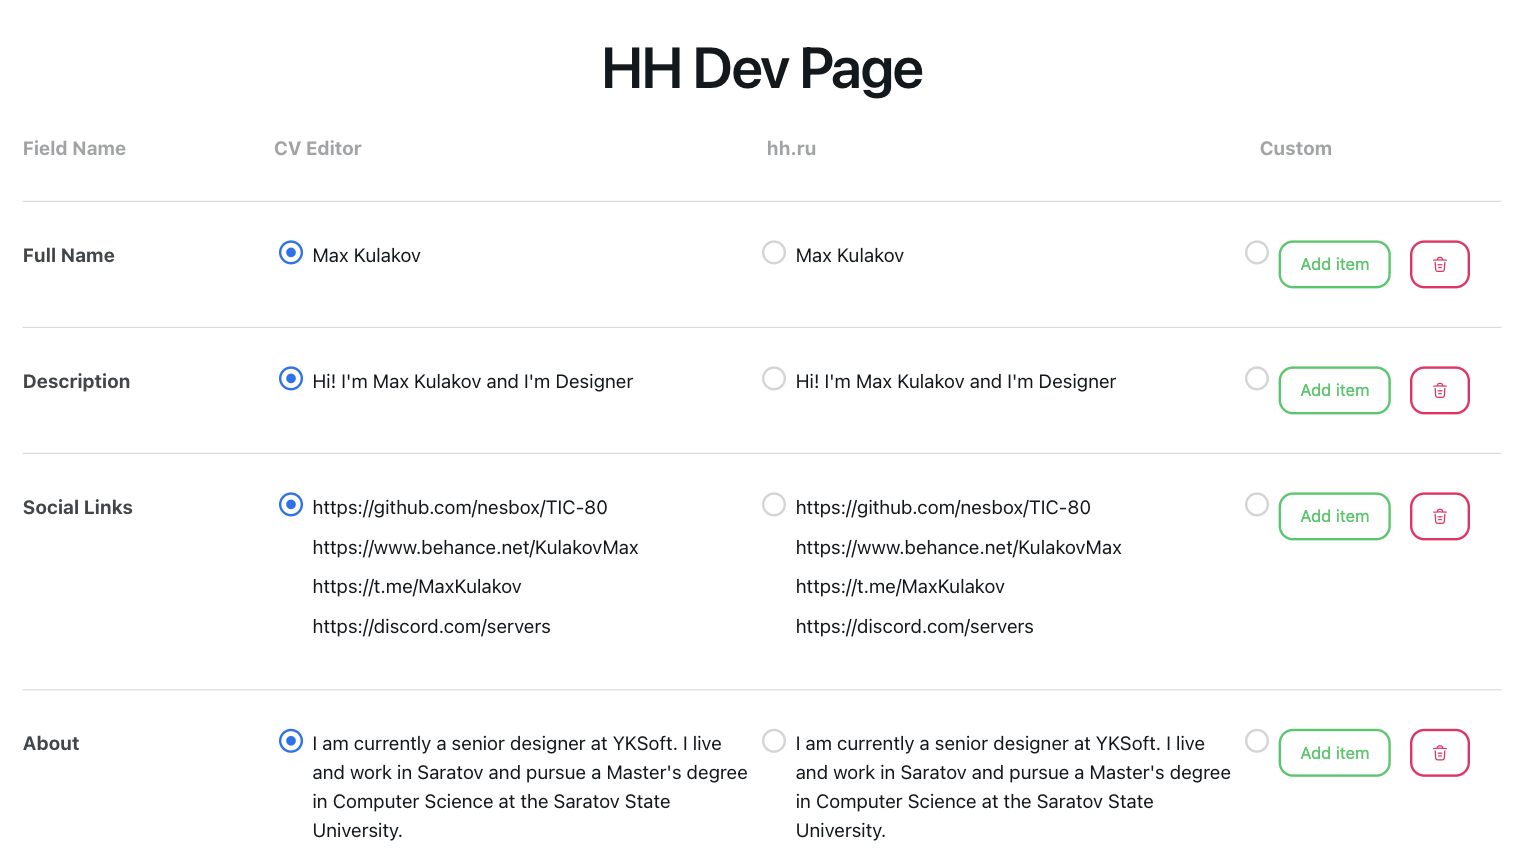
\includegraphics[width=12cm]{images/image-compare-skills.png}
    \caption{\label{fig:5}%
        Страница сравнения навыков}
\end{figure}

В серверной части платформы реализуем API метод для обновления данных резюме на сервисе hh.ru. Для этого в файле api/hh/route.tsx опишем PUT запрос, в заголовок которого передаётся токен пользователя и ссылка на идентификатор резюме, а в тело наименование поля данных с его содержимым. После выполнения запроса в ответ от внутреннего сервера вернётся JSON с кодом и сообщением об успешности выполненной операции.
\begin{minted}[fontsize=\small, breaklines=true, style=bw, linenos]{text}
export async function PUT(req: Request) {
if (resume != null) {
    const body = await req.json()      
    var raw = JSON.stringify( body );
    try { const res = await fetch(`https://api.hh.ru/resumes/${resume}`,{
        method: 'PUT', headers: myHeaders,
        body: raw, redirect: 'follow' })
    return NextResponse.json({ message: "Resume has been updated" });
}}}
\end{minted}

Реализуем страницу обновления навыков, для которой запросим и выведем данные из резюме hh.ru в виде списка тегов с возможностью их удаления из списка. Для этого создадим страницу и инициализируем начальное состояние значений и функцию удаления, проверяющую количество элементов и в случае их полного удаления возвращающего к исходному значению.
\begin{minted}[fontsize=\small, breaklines=true, style=bw, linenos]{text}
export default function ResumePage() {
    const [skill_set, setSkill_set] = React.useState(initialSkills);
    const handleClose = (skillToRemove:any) => {
        setSkill_set(skill_set.filter((skill: any) => 
            skill !== skillToRemove));
        if (skill_set.length === 1) {setSkill_set(initialSkills);}
}};
\end{minted}

Добавим кнопку обновления резюме, по нажатию на которую вызывается функция-обработчик массива строк с преобразованием их к объектному формату JSON и помещающая итоговое значение в тело PUT запроса, отправляющего сообщение через внутрненний сервер на сервис hh.ru.
\begin{minted}[fontsize=\small, breaklines=true, style=bw, linenos]{text}
const skills_body = JSON.parse(JSON.stringify
    (`{"skill_set": [${skill_set.map((x: any) => `"${x}"`)}]}`))
return (
skill_set.map((skill: any, index: any) => (
    <Chip key={index} onClose={() => handleClose(skill)} variant="flat">
        {skill}
    </Chip>
    <Button onClick={updateResume}>Обновить резюме</Button>
)))
\end{minted}

Итоговый вид страницы обновления навыков, содержащей статус изменения списка, редактируемое поле ввода и теги представлен на рисунке~\ref{fig:6}. 
\begin{figure}[!ht]
    \centering
    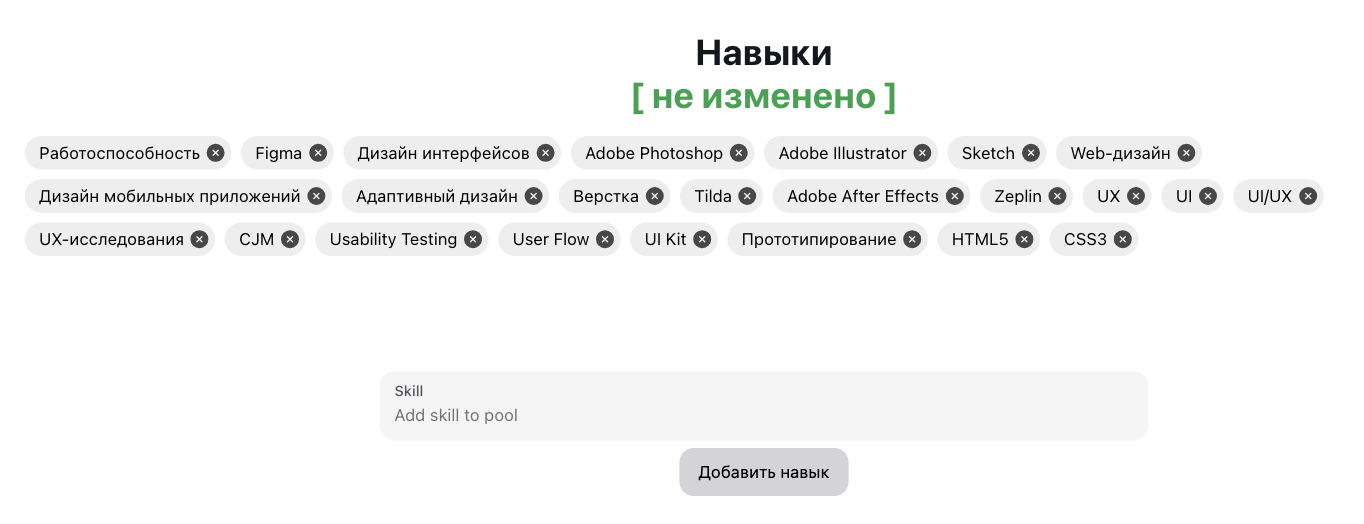
\includegraphics[width=12cm]{images/image-update-skills.png}
    \caption{\label{fig:6}%
        Страница обновления навыков}
\end{figure}





\newpage
\conclusion
В результате проведения исследовательской работы были приобретены навыки анализа качества и эффективности научной литературы в области разработки сервисов с автоматическим обновлением данных, достигнут навык анализирования конкурентных платформ для создания резюме и сформулирован собственный метод масштабирования уже разработанной единой платформы резюме, тем самым было достигнуто полное выполнение поставленных задач. 

В качестве объектов анализа научной литературы выступили статьи по темам разработки клиент-серверного приложения средствами библиотек React JS, TailWind и применением архитектуры Rest API. С учётом проведённого анализа научной литературы были составлены базовые технические требования для масштабирования уже существующего приложения.





% Библиографический список, составленный вручную, без использования BibTeX
%
% \begin{thebibliography}{99}
%   \bibitem{Ione} Источник 1.
%   \bibitem{Itwo} Источник 2
% \end{thebibliography}

% Отобразить все источники. Даже те, на которые нет ссылок.
% \nocite{*}

% Меняем inputencoding на лету, чтобы работать с библиографией в кодировке
% `cp1251', в то время как остальной документ находится в кодировке `utf8'
\inputencoding{cp1251}
\bibliographystyle{gost780uv}
\bibliography{thesis}
\inputencoding{utf8}



% При использовании biblatex вместо bibtex
% \printbibliography

% Окончание основного документа и начало приложений Каждая последующая секция
% документа будет являться приложением
\appendix

\section{Реализация компонента отображения опыта}
\begin{minted}[fontsize=\small, breaklines=true, style=bw, linenos]{text}
"use client";
import * as React from "react";

function diffDates(day_one:any, day_two:any) {
    return (day_one - day_two) / (60 * 60 * 24 * 1000);
};

function getFormatedStringFromDays(numberOfDays:number) {
    numberOfDays = Math.abs(numberOfDays)
    var years = Math.floor(numberOfDays / 365);
    var months = Math.floor(numberOfDays % 365 / 30);
    var yearsDisplay = years > 0 ? 
        years + (years == 1 ? " year " : " years ") : "";
    var monthsDisplay = months > 0 ? 
        months + (months == 1 ? " month " : " months ") : "";
    return yearsDisplay + monthsDisplay; 
}

interface ExperienceItemProps {
    name: string;
    description: string;
    start_date: string;
    end_date: string;
    current_date?: boolean;
}

interface ExperienceProps {
    experience_list: ExperienceItemProps[];
}

export const Experience = (props : ExperienceProps) => {
const experience_item_list = props.experience_list.map((element, index) => {
    const date1 = new Date(element.start_date);
    const date2 = element.current_date ? 
        new Date() : new Date(element.end_date)
    
    return (
        <div key={index} className="grid grid-cols-12 gap-2 mb-4">
            <div className="col-start-1 col-end-3">
                {element.start_date} - {element.end_date} 
                <div className="text-default-500">
                    {getFormatedStringFromDays(diffDates(date1, date2))}
                </div>
            </div>
            <div className="col-start-4 col-end-6">
                {element.name}
            </div>
            <div className="col-start-7 col-end-13">
                {element.description} 
            </div>
        </div>
    )
})
return  <>{experience_item_list}</>
};
\end{minted}




\section{Реализация страницы резюме}
\begin{minted}[fontsize=\small, breaklines=true, style=bw, linenos]{text}
"use client";
import React from "react";
import {Image} from "@nextui-org/react";
import { SocialLink } from "@/components/social-link";
import { Experience } from "@/components/experience";
import { Projects } from "@/components/projects";
import { About } from "@/components/about";

export default function Template1Page() {
const profile_data = require("@/data-template/template-1-data.json");
return (
    <h1 className="h6 text-uppercase text-center pb-4">
        {profile_data.name}
    </h1>
    <p className="text-uppercase text-center pb-2">
        {profile_data.description}
    </p>
    <SocialLink links = {profile_data.social_links}/>
    <div className="grid grid-cols-8 gap-4 mb-12">
        <div className="col-start-3 col-end-7">
            <Image
            isZoomed
            isBlurred
            alt={profile_data.name + " Image"}
            src={profile_data.profile_image}
            />
        </div>
    </div>
    <div className="container pt-5 pb-5 text-left">
        <h2 className="h6 uppercase text-end pb-4" id="about">
            about me
        </h2>
        <About about_text={...profile_data.about}/>
    </div>
    <div className="container pt-5 pb-5 text-left ">
        <h2 className="h6 uppercase text-end pb-4" id="experience">
            education
        </h2>
        <Experience experience_list={...profile_data.education}/>
    </div>
    <div className="container pt-5 pb-5 text-left ">
        <h2 className="h6 uppercase text-end pb-4" id="experience">
            experience
        </h2>
        <Experience experience_list={...profile_data.experience}/>
    </div>
    <div className="container pt-5 pb-5">
        <h2 className="h6 uppercase text-end pb-4" id="projects">
            projects by companies
        </h2>
        <Projects projects_list={...profile_data.projects}/>
    </div>
);}    
\end{minted}




\end{document}
